\documentclass{article}
\usepackage{amsfonts, amsmath, amsthm, amssymb}
\usepackage[urlcolor=blue,linkcolor=black,colorlinks=true]{hyperref}
\hypersetup{
  pdftitle = {Merlin SRP April 2010 Progress Report},
  pdfkeywords = {pdf, hyperref, bookmarks},
  pdfauthor = {Michael Himbeault}
}
\usepackage[headsep=1cm,headheight=50pt]{geometry}
\usepackage[dvips]{graphicx}
\usepackage{subfigure}
\usepackage{lscape}
%input "Nov2009.bib"

\newtheorem{thm}{Theorem}[section]
\newtheorem{cor}[thm]{Corollary}
\newtheorem{lem}[thm]{Lemma}

\newtheorem*{hyp}{Hypothesis}

\theoremstyle{remark}
\newtheorem{remark}[thm]{Remark}

\theoremstyle{definition}
\newtheorem{definition}[thm]{Definition}

\theoremstyle{definition}
\newtheorem{example}{Example}[section]

\theoremstyle{definition}
\newtheorem{algorithm}{Algorithm}[section]

\begin{document}
\bibliographystyle{amsplain}
\title{Merlin SRP - Project Update}
\author{Michael Himbeault}

\maketitle

\section{Custom 'Database' Framework}
In order to have near real-time reaction to network traffic changes, it is necessary to be able to analyze network traffic at line speed. When line speed is on the order of gigabits per second, this becomes far beyond the capabilities of standard solutions. For this reason, a custom data analysis framework was developed.

\subsection{Summary of Existing Solutions}
When reading the following test cases, consider that the optimal memory consumption for 100000 8-byte items is $8\times100000+24\times100000=3.2MiB$. Further, the minimum insertion rate for line-speed processing of flows and DNS packets is approximately 5000 insertions per second at peak, and about 2000 over a 24 hour period.

\begin{description}
\item[Tokyo Cabinet: ] An open source key-value store that initial tests indicate is fast enough but sits at least two orders of magnitude too heavy in memory, ruling it out immediately.
\item[Redis: ] A key-value in-memory database that initial tests indicated was able to handle approximately 150000 very simple insertions per second. Memory consumption was approximately 200MiB for 100000 8-byte items with a key size of 4 bytes.
\item[eXtremeDB: ] A promising product from McObject that offers in-memory and a hybrid (partially in memory, partially on disk/flash such as a FusionIO card) solutions. eXtremeDB is a commercial product and a closed source sample was the only demo environment available to us at the time. Initial tests indicate that it may (or may not) be viable, as tests were somewhat inconclusive.

Some tests show viability in the speed or memory areas, but not in the other, while others failed both criteria.
\item[Any disk-based solution: ] Because of the nature of insertions, a disk-based solution was ruled out almost immediately. While no tests were conducted, research indicates that 25000 insertions per second is a 'reasonable' upper bound for performance metrics. It is trivially easy to exceed this in real-world situations. This rules out systems such as MySQL, Postgre SQL, and others.
\end{description}

\subsection{Performance of Custom ODB Framework}
Testing the custom framework in situations similar to those listed above (a direct correlation is not possible because most of the above are key-value systems, and the ODB framework is not) results in performance metrics of approximately 1-million insertions per second with a memory footprint that can be as low as the theoretical minimum, but with real-world overhead approaching approximately 12 bytes per item.

\subsection{Layout of the ODB Framework}
The ODB framework was based around breaking the problem into two subproblems: data storage, and data indexing. These two problems were tackled independently and the results were merged into what became the ODB framework.

The problem of data storage required a solution that would store piece of arbitrary data in a persistent, secure location that prioritized minimal memory footprint and minimal processing overhead over all else. Two different types of \emph{datastores} were produced with their own benefits and drawbacks.

\begin{description}
\item[Linked List: ] The linked list datastore type is a singly linked list that produces a data overhead of at least 8 bytes per item on a 64-bit system. This type of datastore sacrifices memory efficiency (in the form of the extra 8 bytes per item for the next pointer, as well as any overhead incurred by the \emph{malloc} in use on the system) and some speed (in the form of larger allocs and malloc's overhead on each item's insertion) for ease of deletion, and the fact that the oldest items are always kept at the \emph{tail} of the datastore.

A variation of this datastore type exists that allows it to store variable sized data elements.
\item[Bank: ] The bank datastore type is essentially a list of buckets, where each bucket is the same size. This datastore type sacrifices efficiency of deletion (requiring a far more complicated code path for deletion) for the exceptionally small memory and processing overhead per item.

This datastore can only store pieces of data that are all the same size.
\end{description}

Index tables are then built on top of these and make use of function pointers to determine the individual parameters of each index table.

\subsection{Real World Performance}
The ODB framework is capable of approximately 500000 \emph{combined} insertions and deletions per second on two 3.2GHz CPU cores with 1333MHz RAM with a reasonably sized dataset already in memory. The emphasis on combined insertions and deletions is important as if there are twenty index tables being updated with every piece of data that comes in, then approximately 25000 items can be inserted into the system per second.

\section{Results of Data Analysis}
\subsection{Invalid DNS Packets}
Invalid DNS packets have several properties that separate them immediately from valid DNS packets.

\begin{description}
\item[Ratio of Uniqueness: ] Invalid DNS packets, taken as a whole over a 24 hour period, demonstrate a very different distribution of \emph{uniqueness} than the distribution produced by valid DNS queries. Since talking about the \emph{query string} of an invalid DNS packet is nonsensical, the entire payload of the packet was considered (That is, everything after the UDP header). Analysis indicates that the ratio of the total number of invalid DNS packets to the number of unique payloads is less than 1.5 for the datasets that are on file.

For context, when considering the ratio of the total number of valid DNS queries, to the number of unique query strings, the ratio is significantly greater. Figure \ref{RatioTable} contains the ratios for the known datasets.

This alone is not surprising, quite the contrary in fact as it is expected, however the specifics of the values are interesting. Note the deviation of the two ratios and the lack of direct correlation. This value would be very interesting if it would be tracked over a longer period of time with varying windows.

\item[Query Lengths: ] Invalid DNS packets, because of the data they are expected to carry, unsurprisingly exhibit a very different packet length distribution from valid DNS packets. Figure \ref{LengthPlot} shows the plots of frequency against length (note that the frequency is $\log_{10}$). Again, the length for invalid packets is chosen to be the number of octets contained in the payload of the packet, and valid DNS packets have the number of characters (not Unicode) in the query string.

It is evident that the valid DNS queries cluster close to zero far more tightly than invalid DNS queries. It is also important to note the spike for invalid DNS packets at 1392 bytes. This is the maximum payload for a packet with an MTU of 1434 bytes. It is also worth noting that the invalid DNS graph appears distinctly bimodal when viewed under logarithmic scaling.

\item[Filtering Query Strings: ] It is possible to filter out a large number of the DNS queries using only a few filter rules.
\begin{itemize}
\item Discard facebook.com: Facebook make use of many third-level domains for load balancing the image bandiwdth.
\item Discard in-addr.arpa, ip6.arpa: These are IPv4 and IPv6 reverse lookups.
\item Discard mcafee.com, barracuda.com, mailpolice.com, support-intelligence, surbl.org, uribl.com, rfc-ignorant.org: These TLDs appear to use DNS for much of their spam filtering.
\item Discard anything starting with \#\#. or \#\#\#.: These are in great number and would require a deeper inspection as the TLDs vary widely.
\item Discard anything starting with ns2.: These, while probably not innocuous, are still a large number and should be analyzed separately.
\end{itemize}

This reduces the total number of valid DNS queries left for analysis by up to 95\% (Christmas day) and by as little as 65\% (January 13, 2010).
\end{description}

\begin{figure}
\begin{center}
\begin{tabular}{c|c||c|c}
Invalid & Valid & Invalid & Valid\\
\hline\hline
1.044682&12.037308&1.133203&14.279739\\
1.071997&13.525588&1.090036&16.996146\\
1.112447&15.964914&1.090710&16.968267\\
1.105609&17.689199&1.090108&17.219631\\
1.096777&16.536889&1.098024&16.438949\\
1.139771&13.766609&1.245622&18.564984\\
1.122561&13.715080&1.202785&19.951996\\
1.096424&14.881230&1.096697&19.914346\\
1.092864&14.880821&1.092325&21.566803\\
1.109946&13.446518&1.091545&18.300677\\
1.083557&13.510560&1.070759&15.137681\\
1.081767&14.217730&1.073844&14.185887\\
1.081789&20.157858&1.070302&14.174369\\
1.080215&20.253640&1.066396&13.946848\\
1.087464&18.578653&1.087820&13.912607\\
1.086105&15.100024&1.050857&14.686439\\
1.100218&15.786644&1.088773&14.807836\\
1.098938&16.055668&1.082095&18.460488\\
1.092586&16.439079&1.082948&18.401163\\
1.097468&16.690899&1.138126&18.981257\\
1.113651&14.819052&1.081396&18.900786\\

\end{tabular}
\end{center}
\caption{List of ratios for DNS packets for the known datasets.}\label{RatioTable}
\end{figure}

\begin{landscape}
\begin{figure}
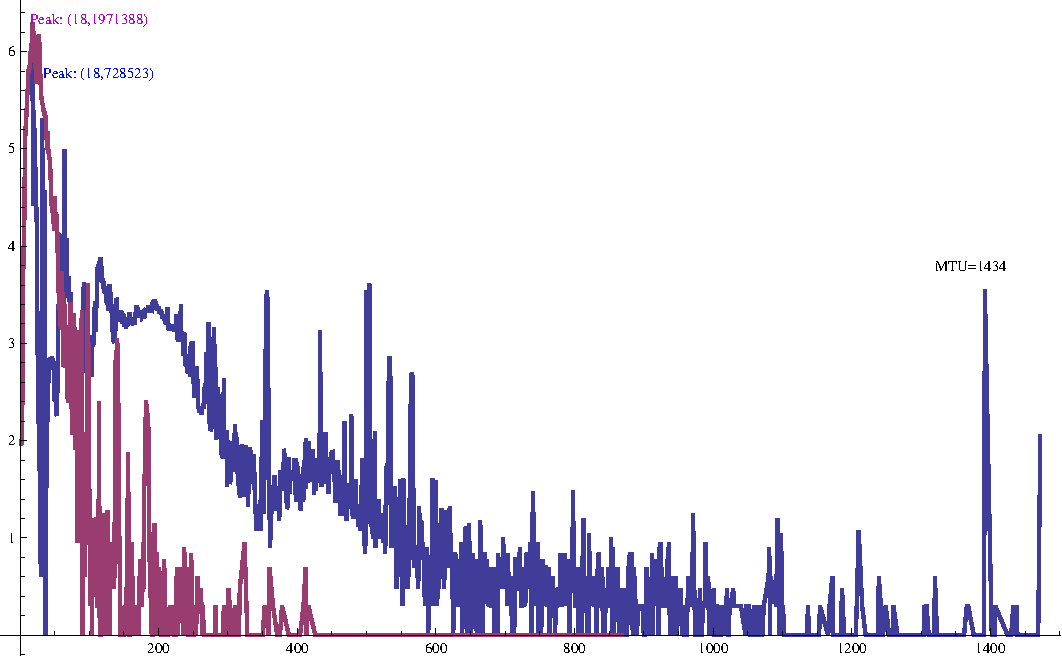
\includegraphics[width=1.4142\textwidth]{LengthPlot.pdf}
\caption{Plots of the frequencies of the lengths of invalid and valid DNS packets. Vertical scale is logarithmic (base 10). Data from Wednesday January 13, 2010. Blue is invalid and purple is valid.}\label{LengthPlot}
\end{figure}
\end{landscape}

\begin{figure}
\subfigure[Time-series plot of the ratios for valid DNS queries.]{
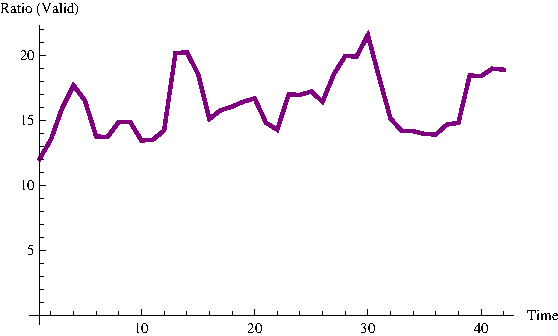
\includegraphics[width=0.5\textwidth]{ValidPlotTime.pdf}}
\subfigure[Time-series plot of the ratios for invalid DNS queries. Observe that the scale is different.]{
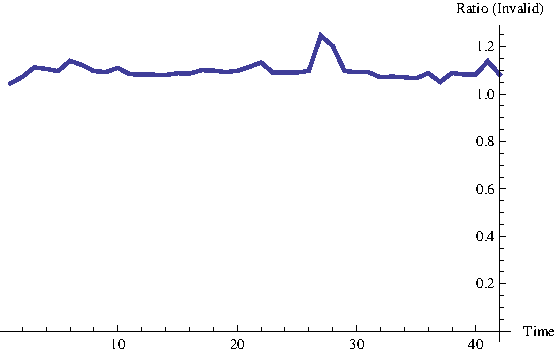
\includegraphics[width=0.5\textwidth]{InvalidPlotTime.pdf}}
\begin{center}
\subfigure[Scatter plot of the invalie and valid ratios, showing the line of best fit and correlation coefficient.]{
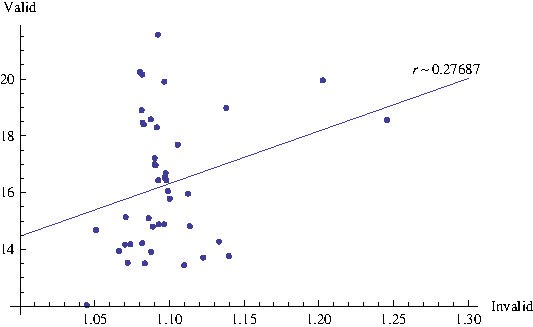
\includegraphics[width=0.5\textwidth]{CorrelationPlot.pdf}}
\end{center}
\end{figure}

\section{Future Analysis}
\begin{itemize}
\item Since the analysis framework is fast enough to sit inline and process at line speed, it would be valuable to get that implemented as soon as possible as it can begin to collect summary data on a daily basis, as well as on various other time frames. Because of the predicted exceptionally slow growth of the number of unique DNS queries, it would be possible to maintain persistent probability data for unique DNS queries.

\item It is expected that if a persistent analysis can be done (by 'priming' the engine with the past data, and then putting it in line) it could detect 0-day anomalies based on the distribution of 'new' DNS queries.

\item As new techniques and trends are established, more advanced analysis can be built on top of this engine that is already processing the data at line speed.
\end{itemize}

% \nocite{*}
% \bibliography{Nov2009}
\end{document}